\documentclass[11pt]{article}
\usepackage{physics}
% NOTE: Add in the relevant information to the commands below; or, if you'll be using the same information frequently, add these commands at the top of paolo-pset.tex file. 
\newcommand{\name}{TA: Hossein Mohammadi}
\newcommand{\email}{hossein.mohammadi.00427@gmail.com}
\newcommand{\classnum}{Advanced Quantum Field Theory}
\newcommand{\subject}{Subject: Renormalization Warm-up, Feynman Rules }
\newcommand{\instructors}{Dr. Amin Faraji}
\newcommand{\assignment}{Mini Set}
\newcommand{\semester}{- Fall 1402}
\newcommand{\duedate}{dd/mm/yyyy}

\input{paolo-pset.tex}

% NOTE: To compile a version of this pset without problems, solutions, or reflections, uncomment the relevant line below.

%\excludeversion{problem}
%\excludeversion{solution}
%\excludeversion{reflection}

\begin{document}	
	
	% Use the \psetheader command at the beginning of a pset. 
	\psetheader
	These are brief questions to warm you up with a quick review of Feynman rules before starting the renormalization section. All these questions could be answered in less than one page by watching the uploaded video or referring to Schwartz’s textbook.
	\section*{Problem 1: LSZ formula}
	
	\begin{problem}
		Express the LSZ formula and its implications. (No formula is needed; just a formal definition and its application and implications in QFT is enough.)
	\end{problem}

	\section*{Problem 2: Momentum Conservation in vertices}

\begin{problem}
	In a general vertex, show momentum conservation, or why $\delta^{(4)}(\sum p_{in} - \sum p_{out})$ appears in Feynman rules.
	
	\noindent
	More specifically, show that by integrating on the vertex position in the figure below, you'll end up with a Dirac delta, which guarantees the momentum conservation. Notice that you just need $e^{\pm ip.x}$ part of the propagator, regardless of its spin.
	
	\begin{figure}[H]
		\centering
		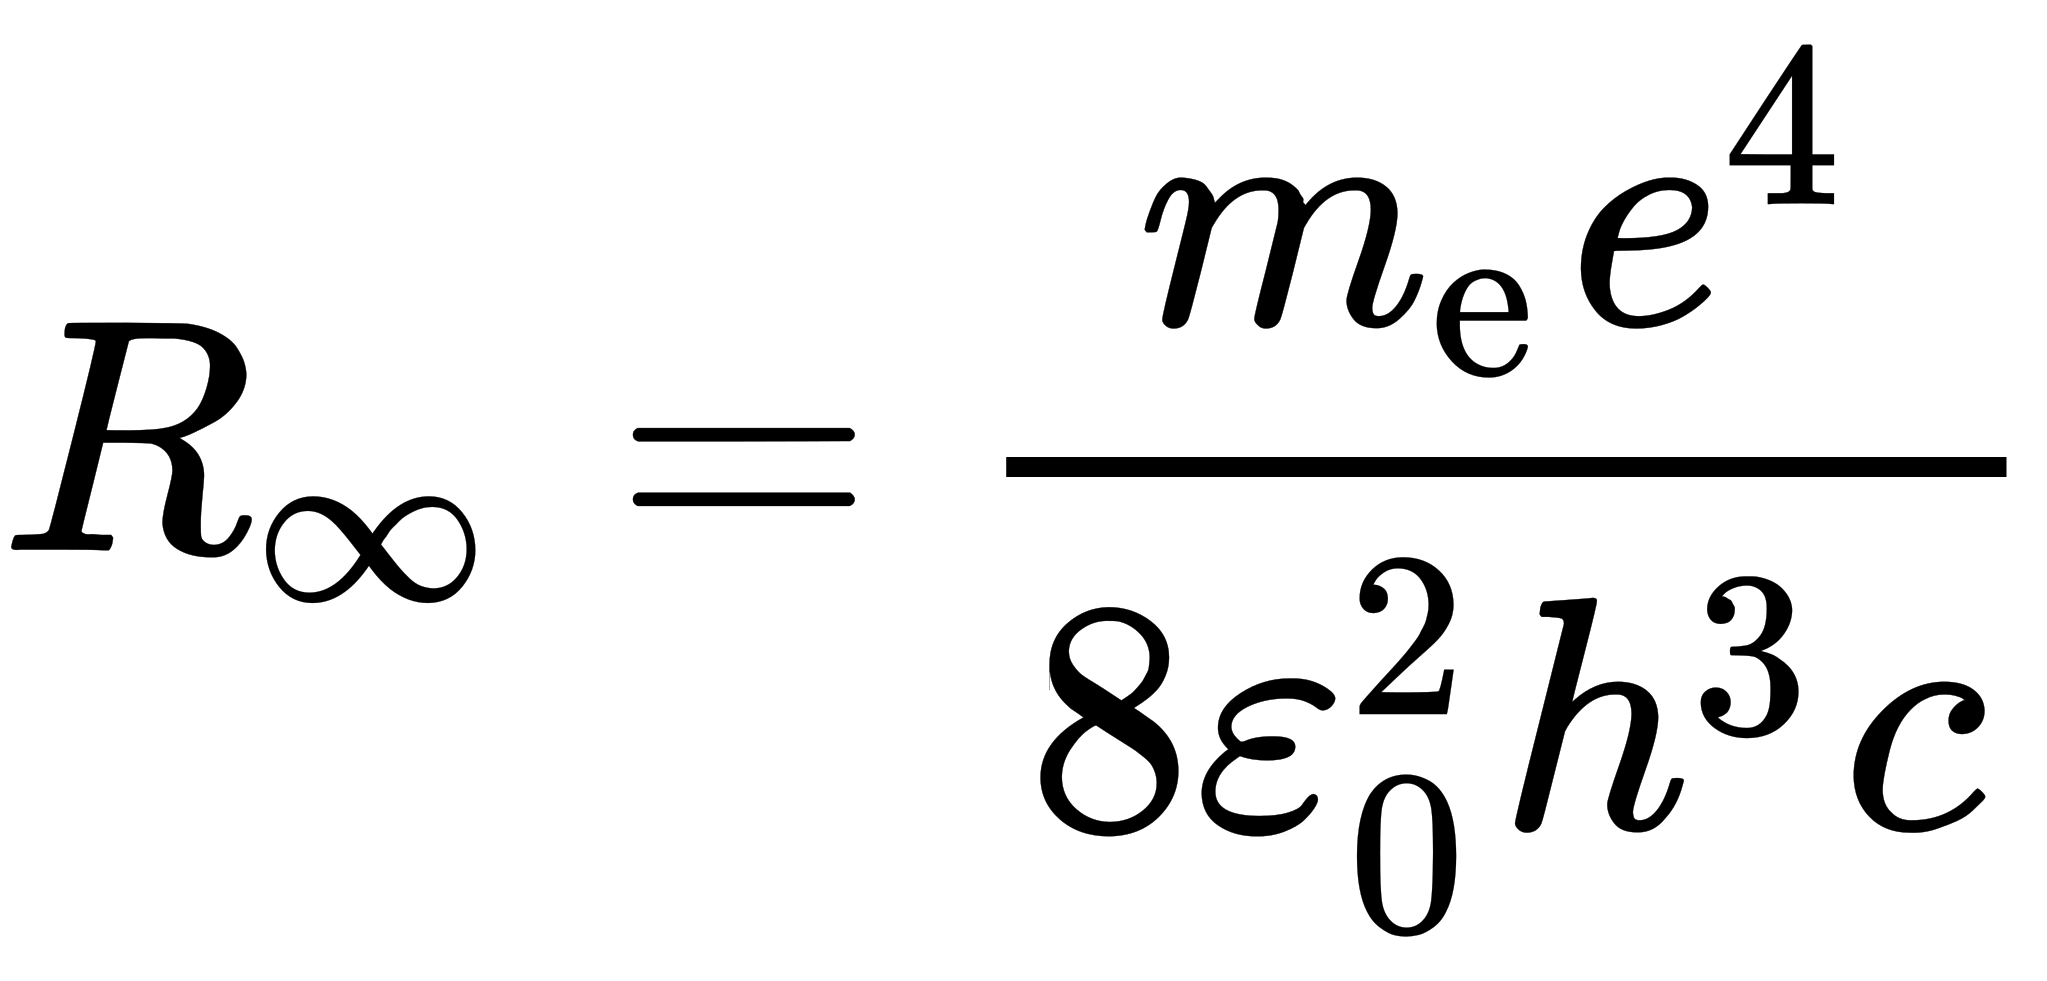
\includegraphics[width=0.4\linewidth]{img/1.png}
		\caption{Momentum conservation - sketch of argument}
	\end{figure}

	
\end{problem}

\newpage
	\section*{Problem 3: Derivative coupling }

\begin{problem}
	Derive the Feynman rule of these two vertices in the figure 2. To be able to do so, I encourage you to look at the uploaded video.
	
	\begin{figure}[H]
		\centering
		\includegraphics[width=0.8\linewidth]{img/2.png}
		\caption{Scalar QED vertices.}
	\end{figure}
	
	
\end{problem}

	\section*{Problem 4: Amplitudes}

\begin{problem}
	Write out the expressions for the amplitude of the following diagrams. The label below each one specifies the theory in which the amplitude should be written.
	
	\begin{figure}[H]
		\centering
		\includegraphics[width=0.8\linewidth]{img/3.png}
		\caption{Amplitudes.}
	\end{figure}
	
	
\end{problem}









\end{document}